\documentclass[10pt]{article}
\usepackage[pdftex]{graphicx, color}
\usepackage{listings}

\usepackage{tikz}
\usetikzlibrary{automata,positioning}

\headheight 8pt \headsep 20pt \footskip 30pt
\textheight 9in \textwidth 6.5in
\oddsidemargin 0in \evensidemargin 0in
\topmargin -.35in

\newcommand {\pts}[1]{({\bf #1 pts})}
\lstset{basicstyle=\small\ttfamily,breaklines=true}

\begin{document}
\begin{center}
\Large CS131 Compilers: Writing Assignment 1\\Due Tuesday, March 27, 2018 at 23:55
\end{center}

\begin{center}
%% Change this:
\LARGE Rong Yuyang - 69850764
\end{center}


This assignment asks you to prepare written answers to questions on
regular languages, finite automata, and lexical analysis.  Each of the
questions has a short answer.  You may discuss this assignment with
other students and work on the problems together.  However, your
write-up should be your own individual work and you should indicate in your submission who you worked
with, if applicable. You should use the Latex template provided at the course web site to write your solution and use the \emph{tikz} package to draw
automata.

\begin{center}
%% Change this:
I worked with: (Name,ID), (Name,ID)...
\end{center}

\begin{enumerate}
  \item \pts{$2\times 3=6$} For each of the follow prompts, write any non-empty sentence:
  \begin{enumerate}
		   \item Name one reason why you would like to learn in this class.

			I want to know how codes are optimized so that I can "reverse engineer" these optimization principles and write better codes.

		   \item Write a question you would like the professor to answer on any topic, from personal opinions to the class material.

		   Would you tell me how parallel compiling is possible and how to make them reliable.

		   \item What do you expect from this class.

		   Fun lectures and a project intensive enough to put to CV.

  \end{enumerate}
  %
  \item \pts{$2\times 4=8$} Write regular expressions for the following languages over the alphabet $\Sigma=\{0,1\}$:
 \begin{enumerate}
		   \item $L_1$: The set of all finite strings containing only three $1's$.
			\[
			L_1 = (0^*10^*)^3
			\]
		   \item $L_2$: The set of all finite strings containing at least three $1's$ and the third character from beginning is $1$.
			\[
		   L_2 = 111(0+1)^* + (10+01)10^*1(0+1)^* + 001(0^*1)^2(0+1)^*
			\]
		   \item $L_3$: The set of all finite strings containing at most three $0's$ and at least two $1's$.
			\[
			%% Your answer here
			\]
		   \item $L_4$: The set of all finite strings which does not contain subsequence $100$.
			\[
			L_4 = 0^*(1^*0)^*
			\]
   \end{enumerate}
   This example illustrates that regular languages are closed under intersection. Note that
   $L_3=L_1\cap L_2$.

  \newpage
   \item \pts{$2\times 4=8$} Draw DFA's for each of the languages $L_1$, $L_2$, $L_3$ and $L_4$ from Question 1.
  \begin{enumerate}
	\item $L_1$.
	\\
	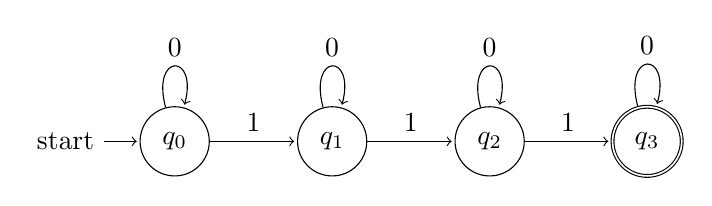
\begin{tikzpicture}[shorten >=1pt,node distance=2cm,on grid,auto]
		\node[state, initial] 	(q_0) 					{$q_0$};
		\node[state] 			(q_1) 	[right=of q_0] 	{$q_1$};
		\node[state] 			(q_2) 	[right=of q_1] 	{$q_2$};
		\node[state, accepting] (q_3) 	[right=of q_2] 	{$q_3$};
		\path[->]
			(q_0) 	edge 	[loop above] 	node 	{0} 	()
					edge 					node 	{1} 	(q_1)
			(q_1) 	edge 	[loop above] 	node 	{0} 	()
					edge 					node 	{1} 	(q_2)
			(q_2) 	edge 	[loop above] 	node 	{0} 	()
					edge 					node 	{1} 	(q_3)
			(q_3) 	edge 	[loop above] 	node 	{0} 	();
	\end{tikzpicture}
	\item $L_2$.
	\\
	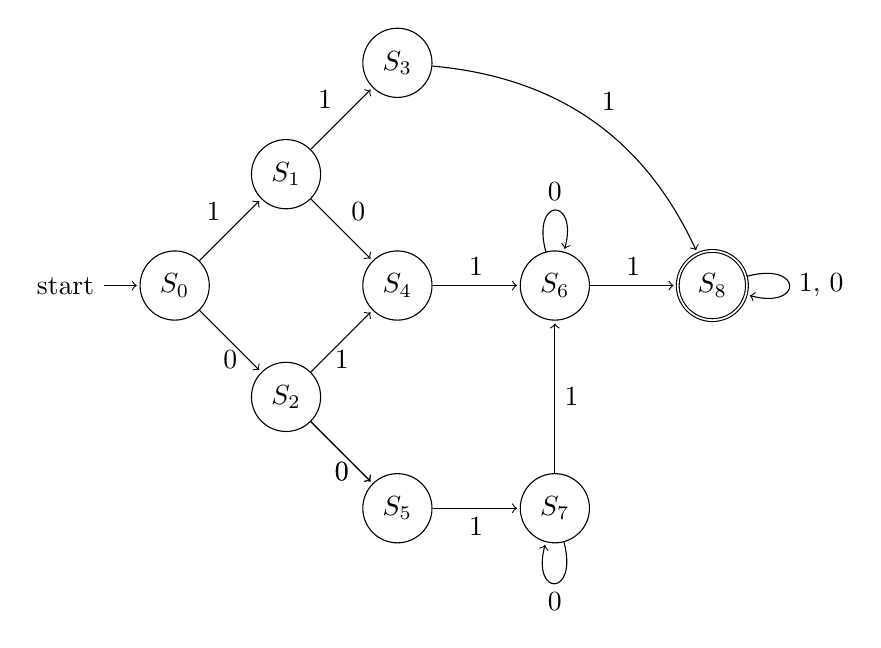
\begin{tikzpicture}[shorten >=1pt,node distance=2cm,on grid,auto]
		\node[state, initial] 	(s0) 						{$S_0$};
		\node[state] 			(s1) 	[above right=of s0]	{$S_1$};
		\node[state] 			(s2) 	[below right=of s0]	{$S_2$};
		\node[state]			(s3) 	[above right=of s1] {$S_3$};
		\node[state] 			(s4) 	[below right=of s1] {$S_4$};
		\node[state] 			(s5) 	[below right=of s2] {$S_5$};
		\node[state] 			(s7) 	[right=of s5]		{$S_7$};
		\node[state] 			(s6) 	[right=of s4] 		{$S_6$};
		\node[state, accepting]	(s8) 	[right=of s6] 		{$S_8$};
		\path[->]
		(s0)	edge	node 			{1} 	(s1)
				edge	node [below]	{0} 	(s2)
		(s1) 	edge 	node			{1}		(s3)
				edge	node			{0}		(s4)
		(s2)	edge 	node [below] 	{1} 	(s4)
				edge 	node [below]	{0}		(s5)
				edge 	node [below]	{0}		(s5)
		(s3)	edge 	[bend left] 	node 			{1}		(s8)
		(s4)	edge	node			{1}		(s6)
		(s5) 	edge 	node [below]	{1}		(s7)
		(s6) 	edge 	[loop above] 	node 			{0}		()
				edge 	node 			{1}		(s8)
		(s7) 	edge 	[loop below]	node 			{0}		()
				edge 	node [right]	{1}		(s6)
		(s8) 	edge 	[loop right] 	node 			{1, 0} 	();
	\end{tikzpicture}
	\item $L_3$.
	\\
	\begin{tikzpicture}[shorten >=1pt,node distance=2cm,on grid,auto]
		%% Your answer here
	\end{tikzpicture}
	 \item $L_4$.
	\\
	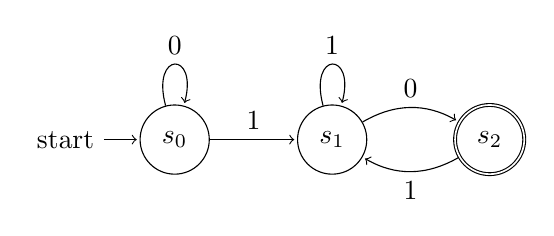
\begin{tikzpicture}[shorten >=1pt,node distance=2cm,on grid,auto]
		\node[state, initial] 	(s0) 					{$s_0$};
		\node[state] 			(s1) 	[right=of s0] 	{$s_1$};
		\node[state, accepting] (s2) 	[right=of s1] 	{$s_2$};
		\path[->]
			(s0) 	edge 	[loop above] 	node 	{0} 	()
					edge 					node 	{1} 	(s1)
			(s1) 	edge 	[loop above] 	node 	{1} 	()	
					edge 	[bend left] 	node 	{0} 	(s2)
			(s2) 	edge 	[bend left] 	node 	{1} 	(s1);
	\end{tikzpicture}
  \end{enumerate}

   \newpage


  \item \pts{$5\times 3=15$} Using the techniques covered in class, transform the following NFAs with $\epsilon$-transitions over the given alphabet $\Sigma$ into DFAs. Note that a DFA must have a transition defined for every state and symbol pair, whereas a NFA need not. You must take this fact into account for your transformations. Hint: Is there a subset of states the NFA transitions to when fed a symbol for which the set of current states has no explicit transition?

  \begin{enumerate}
	\item Original NFA, $\Sigma = \{a, b, c\}$:
	\\
	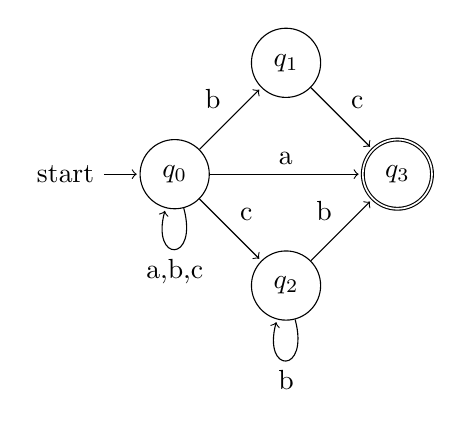
\begin{tikzpicture}[shorten >=1pt,node distance=2cm,on grid,auto]
		\node[state,initial] (q_0)   {$q_0$};
		\node[state] (q_1) [above right=of q_0] {$q_1$};
		\node[state] (q_2) [below right=of q_0] {$q_2$};
		\node[state,accepting](q_3) [below right=of q_1] {$q_3$};
		\path[->]
		(q_0) edge [loop below] node {a,b,c} ()
			  edge  node  [above] {a} (q_3)
			  edge  node  {b} (q_1)
			  edge  node  {c} (q_2)
		(q_1) edge  node  {c} (q_3)
		(q_2) edge  node  {b} (q_3)
			  edge  [loop below] node  {b} ();
	\end{tikzpicture}
	\\
	DFA:
	\\
	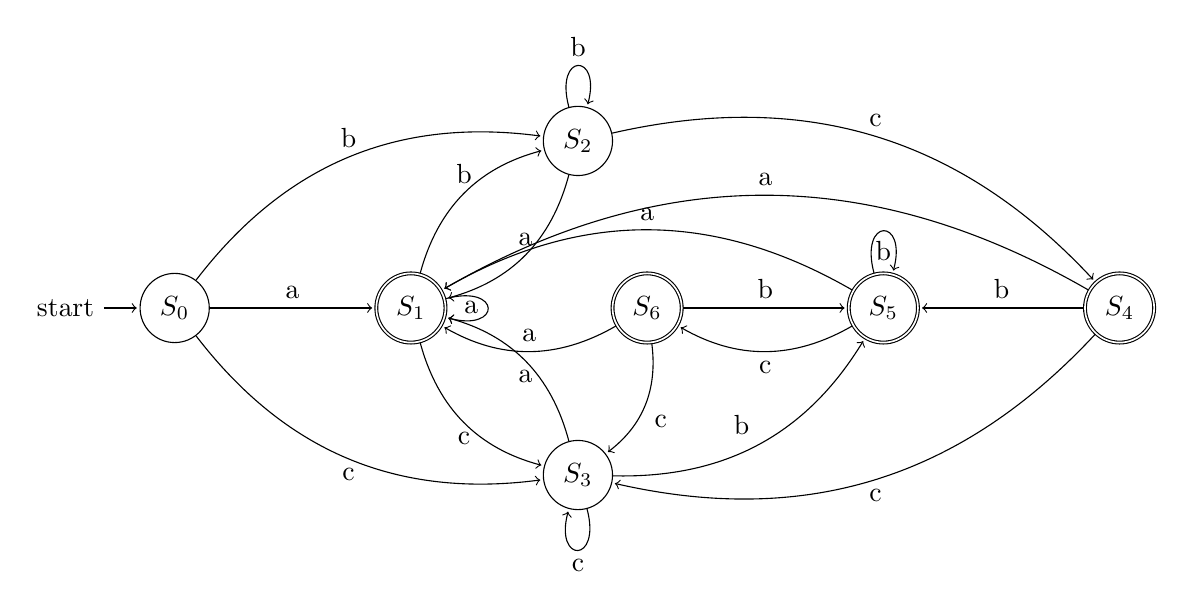
\begin{tikzpicture}[shorten >=1pt,node distance=3cm,on grid,auto]
		\node[state, initial] 	(s0) 						{$S_0$};
		\node[state, accepting]	(s1) [right=of s0] 			{$S_1$};
		\node[state] 			(s2) [above right=of s1] 	{$S_2$};
		\node[state] 			(s3) [below right=of s1] 	{$S_3$};
		\node[state, accepting]	(s6) [right=of s1] 			{$S_6$};
		\node[state, accepting]	(s5) [right=of s6] 			{$S_5$};
		\node[state, accepting]	(s4) [right=of s5] 			{$S_4$};
		\path[->]
		(s0)	edge					node 				{a} 	(s1)
				edge 	[bend right] 	node 	[below] 	{c} 	(s3)
				edge 	[bend left] 	node 	[above] 	{b} 	(s2)
		(s1) 	edge 	[loop right] 	node	[left]		{a} 	()
				edge 	[bend left] 	node 	[above] 	{b} 	(s2)
				edge 	[bend right] 	node 	[below] 	{c}		(s3)	
		(s2) 	edge 	[bend left]	node 	[above] 	{a} 	(s1)
				edge 	[loop above] 	node 				{b}		()
				edge 	[bend left]		node 	[above] 	{c}		(s4)
		(s3) 	edge 	[bend right] 	node 	[below] 	{a} 	(s1)
				edge 	[bend right]	node 				{b}		(s5)
				edge 	[loop below] 	node 	[below]		{c} 	()
		(s5) 	edge 	[loop above] 	node 	[below]		{b} 	()
				edge 	[bend right] 	node 	[above] 	{a}		(s1)
				edge 	[bend left]		node 	[below]		{c} 	(s6)
		(s6) 	edge 	[bend left] 	node 	[above] 	{a}		(s1)
				edge 					node 				{b}		(s5)
				edge 	[bend left] 	node 				{c}		(s3)
		(s4) 	edge 	[bend right] 	node 	[above] 	{a}		(s1)
				edge 					node 	[above] 	{b}		(s5)
				edge 	[bend left]		node 	[below] 	{c}		(s3);
 	\end{tikzpicture}
	\item Original NFA, $\Sigma = \{a, b, c\}$:
	\\
	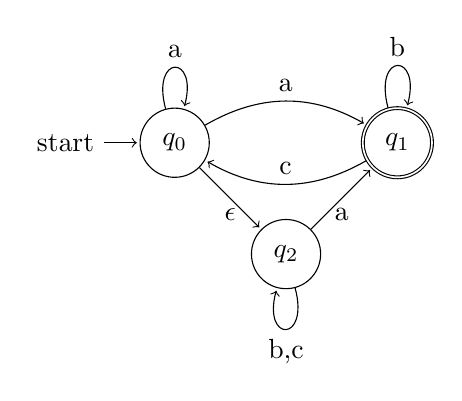
\begin{tikzpicture}[shorten >=1pt,node distance=2cm,on grid,auto]
		\node[state,initial] (q_0)   {$q_0$};
		\node[state] (q_2) [below right=of q_0] {$q_2$};
		\node[state,accepting] (q_1) [above right=of q_2] {$q_1$};
		\path[->]
		(q_0) edge [loop above] node {a} ()
			  edge [bend left] node  {a} (q_1)
			  edge  node [below] {$\epsilon$} (q_2)
		(q_1) edge [loop above] node {b} ()
			  edge [bend left] node [above] {c} (q_0)
		(q_2) edge node [below] {a} (q_1)
			  edge [loop below] node  {b,c} ();
	\end{tikzpicture}
	\\
	DFA:
	\\
	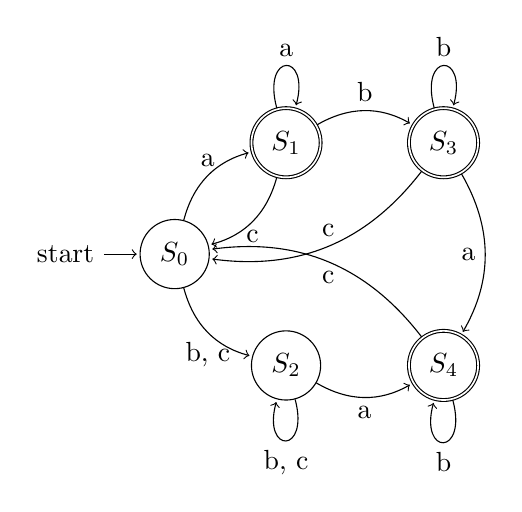
\begin{tikzpicture}[shorten >=1pt,node distance=2cm,on grid,auto]
		\node[state, initial] 	(S0) 						{$S_0$};
		\node[state, accepting] (S1) [above right=of S0]	{$S_1$};
		\node[state] 			(S2) [below right=of S0] 	{$S_2$};
		\node[state, accepting] (S3) [right=of S1] 			{$S_3$};
		\node[state, accepting] (S4) [right=of S2] 			{$S_4$};
		\path[->]
		(S0) 	edge 	[bend left] 	node 	[above] 	{a} 	(S1)
				edge 	[bend right]	node 	[below]		{b, c}	(S2)
		(S1) 	edge 	[bend left] 	node 	[below] 	{c} 	(S0)
				edge 	[loop above] 	node 	[above]		{a}		()
				edge 	[bend left]		node 				{b}		(S3)
		(S2) 	edge 	[loop below] 	node 	[below] 	{b, c} 	()
				edge 	[bend right]	node 	[below]		{a} 	(S4)
		(S3) 	edge 	[bend left] 	node 	[above] 	{c} 	(S0)
				edge 	[loop above] 	node 	[above] 	{b} 	()
				edge 	[bend left]		node 	[left]	 	{a} 	(S4)
		(S4) 	edge 	[loop below] 	node 	[below] 	{b} 	() 	
				edge 	[bend right] 	node 	[below] 	{c} 	(S0);
	\end{tikzpicture}
	\item Original NFA, $\Sigma = \{a, b,c\}$:
	\\
	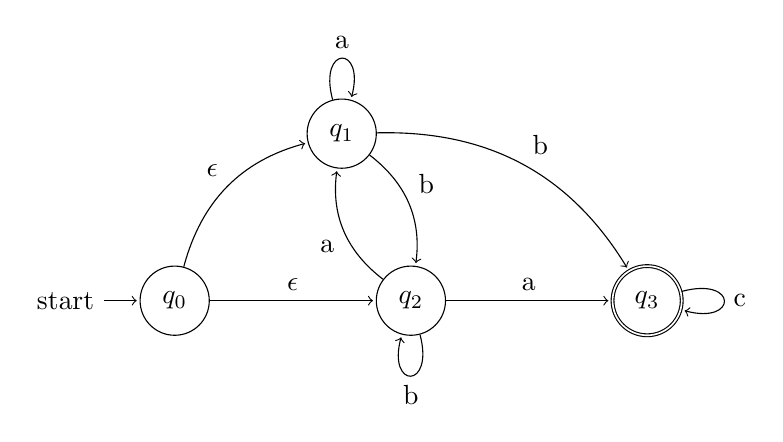
\begin{tikzpicture}[shorten >=1pt,node distance=3cm,on grid,auto]
		\node[state,initial] (q_0)   {$q_0$};
		\node[state] (q_1) [above right=of q_0] {$q_1$};
		\node[state] (q_2) [right=of q_0] {$q_2$};
		\node[state,accepting] (q_3) [right=of q_2] {$q_3$};
		\path[->]
		(q_0) edge [bend left] node  {$\epsilon$} (q_1)
			  edge node  {$\epsilon$} (q_2)
		(q_1) edge [loop above] node {a} ()
			  edge [bend left] node {b} (q_3)
			  edge [bend left] node {b} (q_2)
		(q_2) edge [loop below] node {b} ()
			  edge node {a} (q_3)
			  edge [bend left] node {a} (q_1)
		(q_3) edge [loop right] node {c} ();
	\end{tikzpicture}
	\\
	DFA:
	\\
	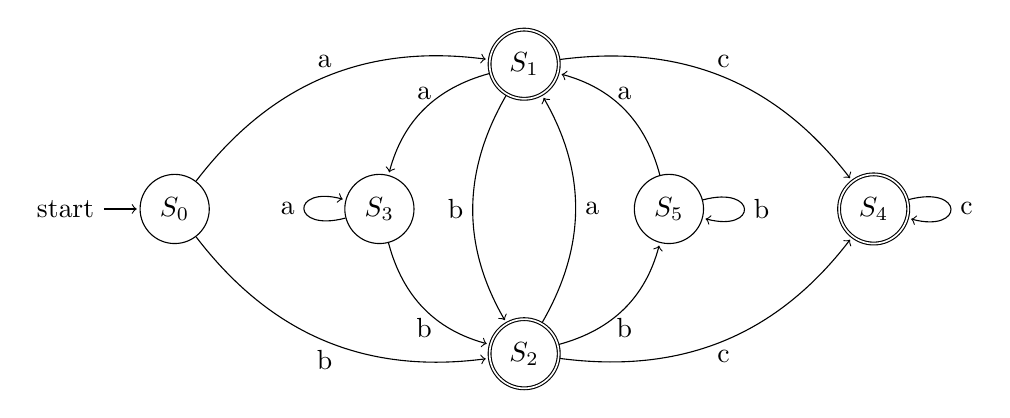
\begin{tikzpicture}[shorten >=1pt,node distance=2.6cm,on grid,auto]
		\node[state, initial] 	(s0) 						{$S_0$};
		\node[state] 			(s3) [right=of s0] 			{$S_3$};
		\node[state, accepting] (s1) [above right=of s3] 	{$S_1$};
		\node[state, accepting] (s2) [below right=of s3] 	{$S_2$};
		\node[state] 			(s5) [above right=of s2] 	{$S_5$};
		\node[state, accepting] (s4) [right=of s5] 			{$S_4$};
		\path[->]
		(s0) 	edge 	[bend left] 	node 	[above] 	{a} 	(s1)
				edge 	[bend right] 	node 	[below] 	{b}		(s2)
		(s1) 	edge 	[bend right] 	node 	[left]	 	{b}		(s2)
				edge 	[bend right] 	node 	[above] 	{a} 	(s3)
				edge 	[bend left] 	node 	[above] 	{c} 	(s4)
		(s2)	edge 	[bend right]	node 	[right] 	{a} 	(s1)
				edge	[bend right] 	node 	[below] 	{b} 	(s5)
				edge 	[bend right] 	node 	[below] 	{c} 	(s4)
		(s3) 	edge 	[loop left] 	node 	[left] 		{a} 	()
				edge 	[bend right] 	node 	[below]		{b}		(s2)
		(s5) 	edge	[bend right] 	node 	[above] 	{a} 	(s1)
				edge 	[loop right] 	node 	[right] 	{b} 	()
		(s4) 	edge 	[loop right] 	node 	[right] 	{c} 	();

	\end{tikzpicture}
  \end{enumerate}

   \newpage
  \item \pts{$13$} Draw the NFA for the set of all strings over the alphabet $\Sigma = \{a,b\}$, where both $a$ and $b$ occur even times.
Examples of strings that should be accepted by this NFA: abbabbbbaa, baabaaabaaaaab.
Examples of strings that should \textbf{not} be accepted: ababb, abbbabba.
	\\
	\\
		Now I already knows that I can construct even As and Bs respectively:
		$	L_a = b^*(ab^*a)^*  $
		$	L_b = a^*(ba^*b)^*  $
		But the problem is how can I use DFA to do $ L_a \cap L_b$?
	\begin{tikzpicture}[shorten >=1pt,node distance=2cm,on grid,auto]

	\end{tikzpicture}

  \newpage
   \item \pts{$5$} Consider the following tokens and their associated regular expressions, given as a \textbf{flex} scanner specification:

  \begin{lstlisting}
	%%
	(if)                    {printf("IF");}
	(0*1|1*0)               {printf("PS");}
	[0-9]+                  {printf("NUM");}
	[a-zA-Z0-9]+            {printf("ID");}
	[ ]                     {}
  \end{lstlisting}

  Give an input to this scanner such that the output string is $\tt (NUM^{\rm 2} IF^{\rm 2} ID^{\rm 3} PS)^{\rm 2}$, where $\tt A^i$ denotes {\tt A} repeated {\tt i} times.   (And, of course, the parentheses are not part of the output.)  You may use similar shorthand notation in your answer.
  \[
	((234\ )^2(if\ )^2(a\ )^301)^2
  \]

  \newpage
  \item \pts{$5$} Draw the minimal DFA of the DFA constructed in Question 4(c).
   \\
	\\
	\begin{tikzpicture}[shorten >=1pt,node distance=2cm,on grid,auto]
		%% Your answer here
	\end{tikzpicture}

\end{enumerate}
\end{document}

